%!TEX root = ../../main.tex
\section{Macromolecular X-ray crystallography (MX)}
\label{sec:X-ray crystallography}

    Macromolecular X-ray crystallography (MX) is by far the most common technique used for solving the atomic structure of 3D macromolecules.
    As of 14th June 2016 the Protein Data Bank (PDB) contained 119,480 structures and just over 89\% of those structures were solved by MX.
    Despite the dominance of MX, there are many stages in the structure solution pipeline that present their own challenges.
    The typical protein structure solution pipeline in X-ray crystallography is outlined in Figure~\ref{fig:Crystallography-pipeline} \cite{garman2014}.

    \begin{figure}
        \centering
        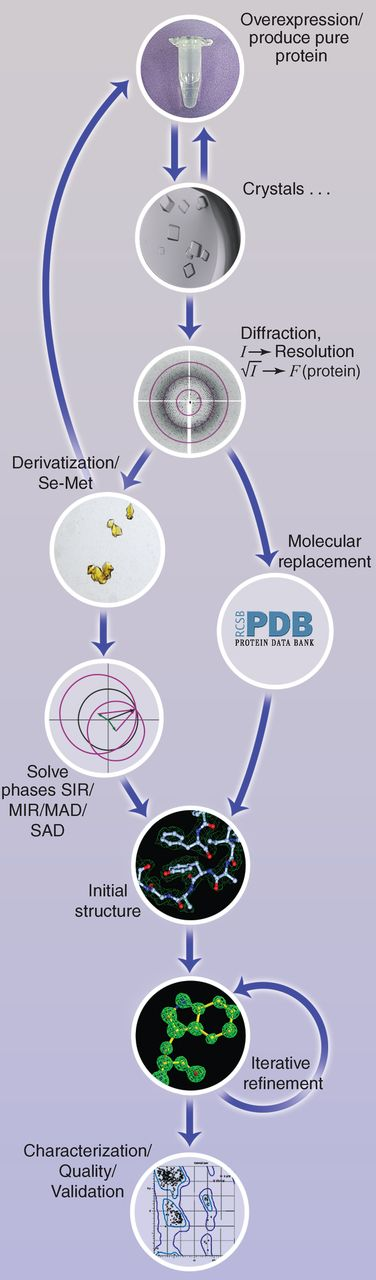
\includegraphics[width=0.4\textwidth]{figures/introduction/crystallography_pipeline.jpg}
        \caption[MX structure solution pipeline.]{Typical protein structure solution pipeline in X-ray crystallography \cite{garman2014}.}
        \label{fig:Crystallography-pipeline}
    \end{figure}

    \subsection{Producing a protein crystal}
    \label{sub:Producing a protein crystal}
        When a particular protein target has been identified, the first step is to produce it in an appropriate expression system.
        \textit{E.coli} is the most common system since it is cheap, fast and produces higher quantities of protein compared to other systems \cite{rai2001expression}.
        However other expression systems such as yeast, insect and mammalian cells are used when bacterial systems are not suitable e.g. bacterial cells lack the capacity to perform certain types of post-translational modification such as glycosylation.
        The target protein is generally not the only product formed during the expression phase, so it has to be isolated.
        The process of isolating the target protein is known as purification, methods for which include filtration and chromatography \cite{graslund2008protein}.
        The next step is crystallisation, which is generally regarded as the major bottleneck in crystallography \cite{garman2014}.
        At this stage of the pipeline, a solution containing the purified target protein is mixed with a precipitant solution to achieve suitable chemical and environmental conditions for crystallogenesis.
        However, in general the exact conditions for crystallogenesis for a given protein are unknown, hence many laboratories use robots to screen multiple conditions in the hope of finding the correct one(s) \cite{luft2007efficient}.

    \subsection{Crystals}
    \label{sub:Crystals}
        A conventional crystal is essentially a 3D repeating array of identical subunits known as unit cells (Figure~\ref{fig:Unit cells as building blocks}).
        A unit cell is defined by six parameters - $a, b, c, \alpha, \beta, \gamma$ (Figure~\ref{fig:Unit cell definition}).
        $a, b, c$ represent the lengths of the edges of the unit cells and $\alpha, \beta, \gamma$ are the angles between them \cite{drenth2012}.
        \begin{figure}[H]
            \centering
            \begin{subfigure}[b]{0.45\textwidth}
                    \centering
                    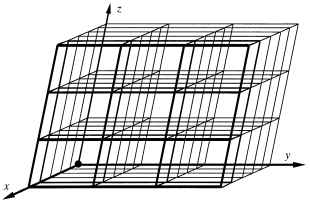
\includegraphics[width=\textwidth]{figures/introduction/unitcellsbuildingblocks.png}
                    \caption{}
                    \label{fig:Unit cells as building blocks}
            \end{subfigure}
            \qquad
            \begin{subfigure}[b]{0.4\textwidth}
                    \centering
                    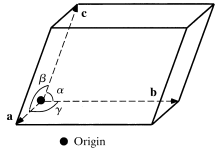
\includegraphics[width=\textwidth]{figures/introduction/unitcelldefinition.png}
                    \caption{}
                    \label{fig:Unit cell definition}
            \end{subfigure}
            \caption[Lattice definition.]{(a) Crystals are formed by repeating unit cells related by translations in all 3 dimensions.
            The intersection points of the lines are the lattice points.
            (b) A single unit cell with axes $\bs{a}, \bs{b}$ and $\bs{c}$, with angles between them $\alpha, \beta$ and $\gamma$. \cite{drenth2012}}
    		\label{fig:Introduction-Unit Cells}
        \end{figure}
        If $a, b, c$ are viewed as directional vectors (vectors will be generally represented by lowercase bold letters {$\bs{a}, \bs{b}, \bs{c}$}) instead of physical unit cell lengths, and only integer multiples of them are considered, then the resulting set of points is referred to as a (Bravais) lattice.
        Visually the lattice is a set of points, which can be viewed as the points where the edges of the unit cells intersect each other in Figure~\ref{fig:Unit cells as building blocks}.
        Mathematically this is equivalent to:
        \begin{equation}
            \{n_1 \bs{a} + n_2 \bs{b} + n_3 \bs{c}\ |\ n_1, n_2, n_3 \in \mathbb{N} \},
            \label{eq:Bravais Lattice}
        \end{equation}
        where $\mathbb{N}$ denotes the set of natural numbers $\{$ 0, 1, 2, 3,$\ldots \}$ (Note: sometimes the set of natural numbers is defined as excluding 0 but here it is included).
        The terms `crystal' and `lattice' are sometimes used interchangeably because they are very closely related.
        However, the distinction between the physical crystal and the hypothetical lattice is made clear by noticing that the set defined in equation \ref{eq:Bravais Lattice} implies that the array of lattice points is infinite, whereas the physical crystal is not.
        Despite this distinction, the properties of lattices are applicable to crystals.

        There are different types of lattices which are defined by their lattice (axial) system and their types (centerings) (examples given in Figure~\ref{fig:2D Bravais lattices}).
        In three dimensions there are 7 lattice systems and 7 lattice types, and these combine to make the set of 14 Bravais Lattices.
        (Note: a stricter way to define the 14 possible Bravais lattices is to realise that two lattices are equivalent if their symmetry groups are isomorphic.
        Bravais' original criterion only classifies 11 types of lattice \cite{pitteri1996definition}).
        \begin{figure}
            \centering
            \begin{subfigure}[b]{0.45\textwidth}
                    \centering
                    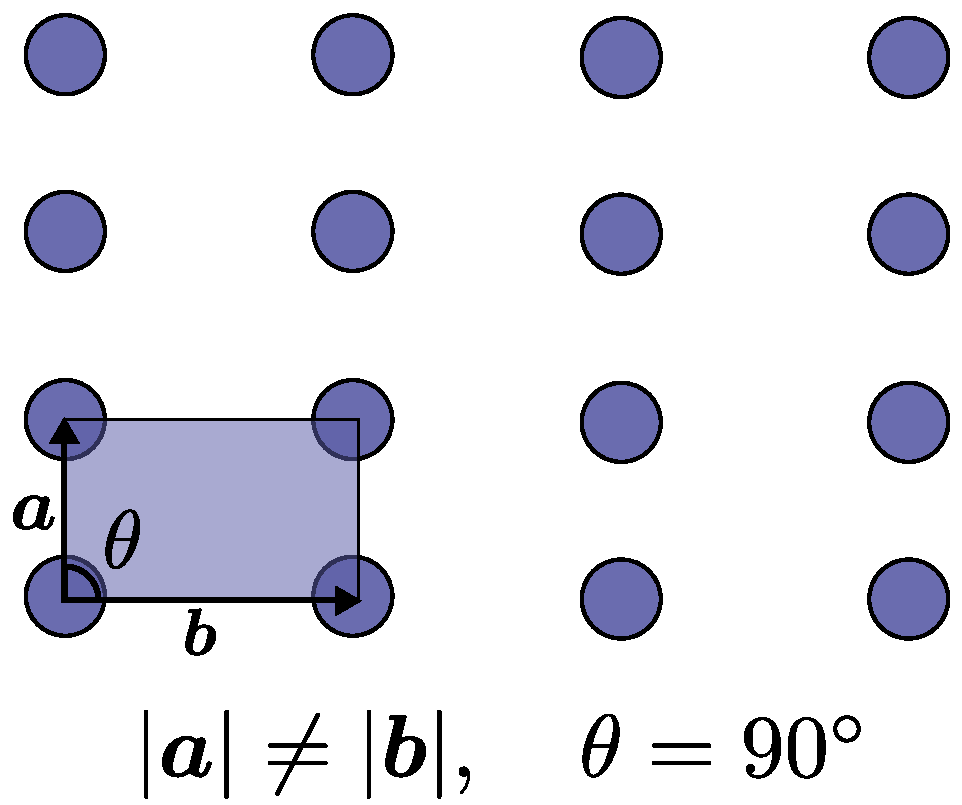
\includegraphics[width=\textwidth]{figures/introduction/rectangularbravaislattice.pdf}
                    \caption{}
                    \label{fig:2D rectangular Bravais lattice}
            \end{subfigure}
            \qquad
            \begin{subfigure}[b]{0.45\textwidth}
                    \centering
                    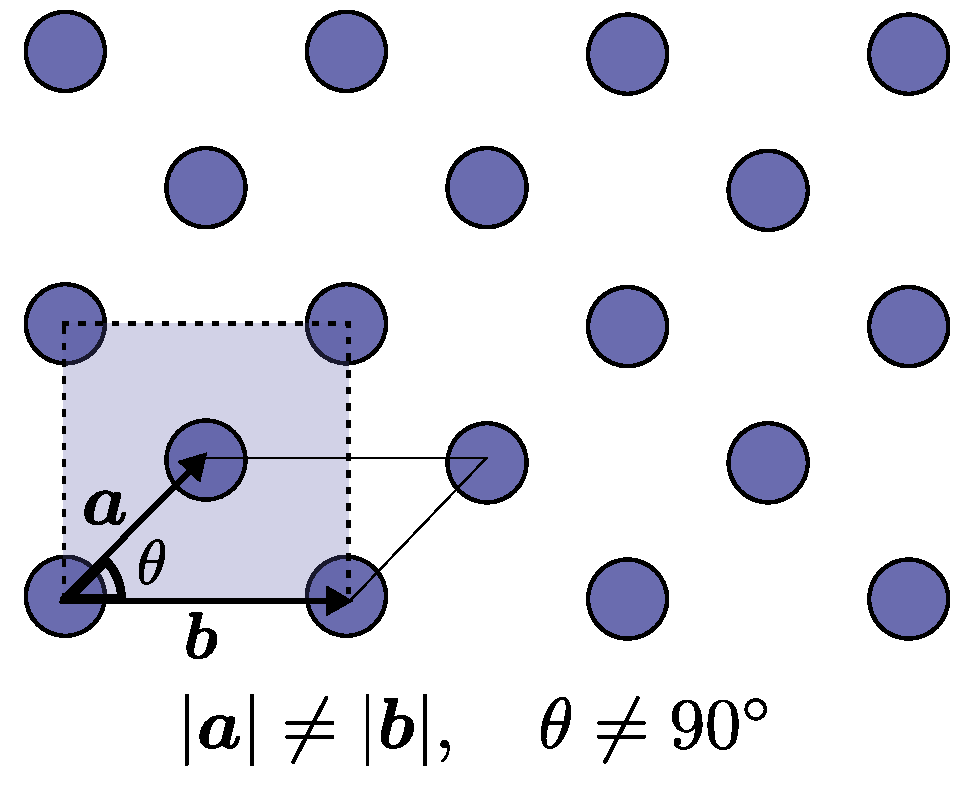
\includegraphics[width=\textwidth]{figures/introduction/centredrectangularbravaislattice.pdf}
                    \caption{}
                    \label{fig:2D centred rectangular Bravais lattice}
            \end{subfigure}
            \caption[Two dimensional Bravais lattices.]{Two dimensional Bravais lattices. (a) Rectangular lattice system with no centering. (b) Centred rectangular lattice system.}
    		\label{fig:2D Bravais lattices}
        \end{figure}

        Thus far, only translational symmetries have been considered for unit cells in a crystal.
        These transformations move every point in space from their original position.
        However, Bravais lattices also possess symmetry operations that leave at least one point in space fixed.
        These are called the point group symmetries and consist of reflections and rotations.
        Protein molecules are chiral and hence symmetry operations that reverse the chirality of the molecule are not allowed for protein crystals (these correspond to the reflections - symmetry operations for which the determinant of the transformation matrix is equal to -1).
        Further to this, the crystallographic restriction theorem only allows for 2, 3, 4, and 6 fold rotations \cite{coxeter1973regular}.
        This leaves only 11 enantiomorphic point groups allowed for protein crystals \cite{drenth2012}.

        The combination of fractional translations along a unit cell axis with rotations result in screw axis symmetry operations.
        When these operations are combined with the point group, the resulting set of operations is referred to as the space group.
        There are 65 enantiomorphic space groups allowed for protein crystals \cite{drenth2012}.

    \subsection{The diffraction experiment}
    \label{sub:The diffraction experiment}
        The final experimental stage of the structure solution pipeline is the data collection.
        Once a suitable crystal composed of the target protein has been grown, diffraction data are collected using a method that will also keep the crystal hydrated in the solution in which it was grown: the mother liquor.
        It is then mounted and irradiated with a beam of intense X-rays (energy usually between 6 and 18\,keV), typically whilst being rotated, although other collection protocols are becoming increasingly common (e.g. helical scans).
        Over a small angular rotation range, the diffracted X-ray photons are collected on a position sensitive detector and produce a diffraction pattern (a diffraction image) that is unique to that protein (Figure~\ref{fig:Insulin diffraction image}).
        The spots that are observed on the images are known as reflections. These observations are in fact the intensities of the reflections.
        The goal of the data collection experiment is to accurately measure the intensities of as many reflections (unique and multiplicitous) as possible.
        The space that contains these reflections is known as reciprocal space.
        Therefore to sample as much of reciprocal space as possible, multiple diffraction patterns are collected as the crystal rotates (often the number of images range in the hundreds).
        Understanding how the diffraction of the X-ray photons arise from their interaction with the atoms in the protein crystal allows crystallographers to interpret the pattern and solve the atomic structure of the protein.
        \begin{figure}
            \centering
            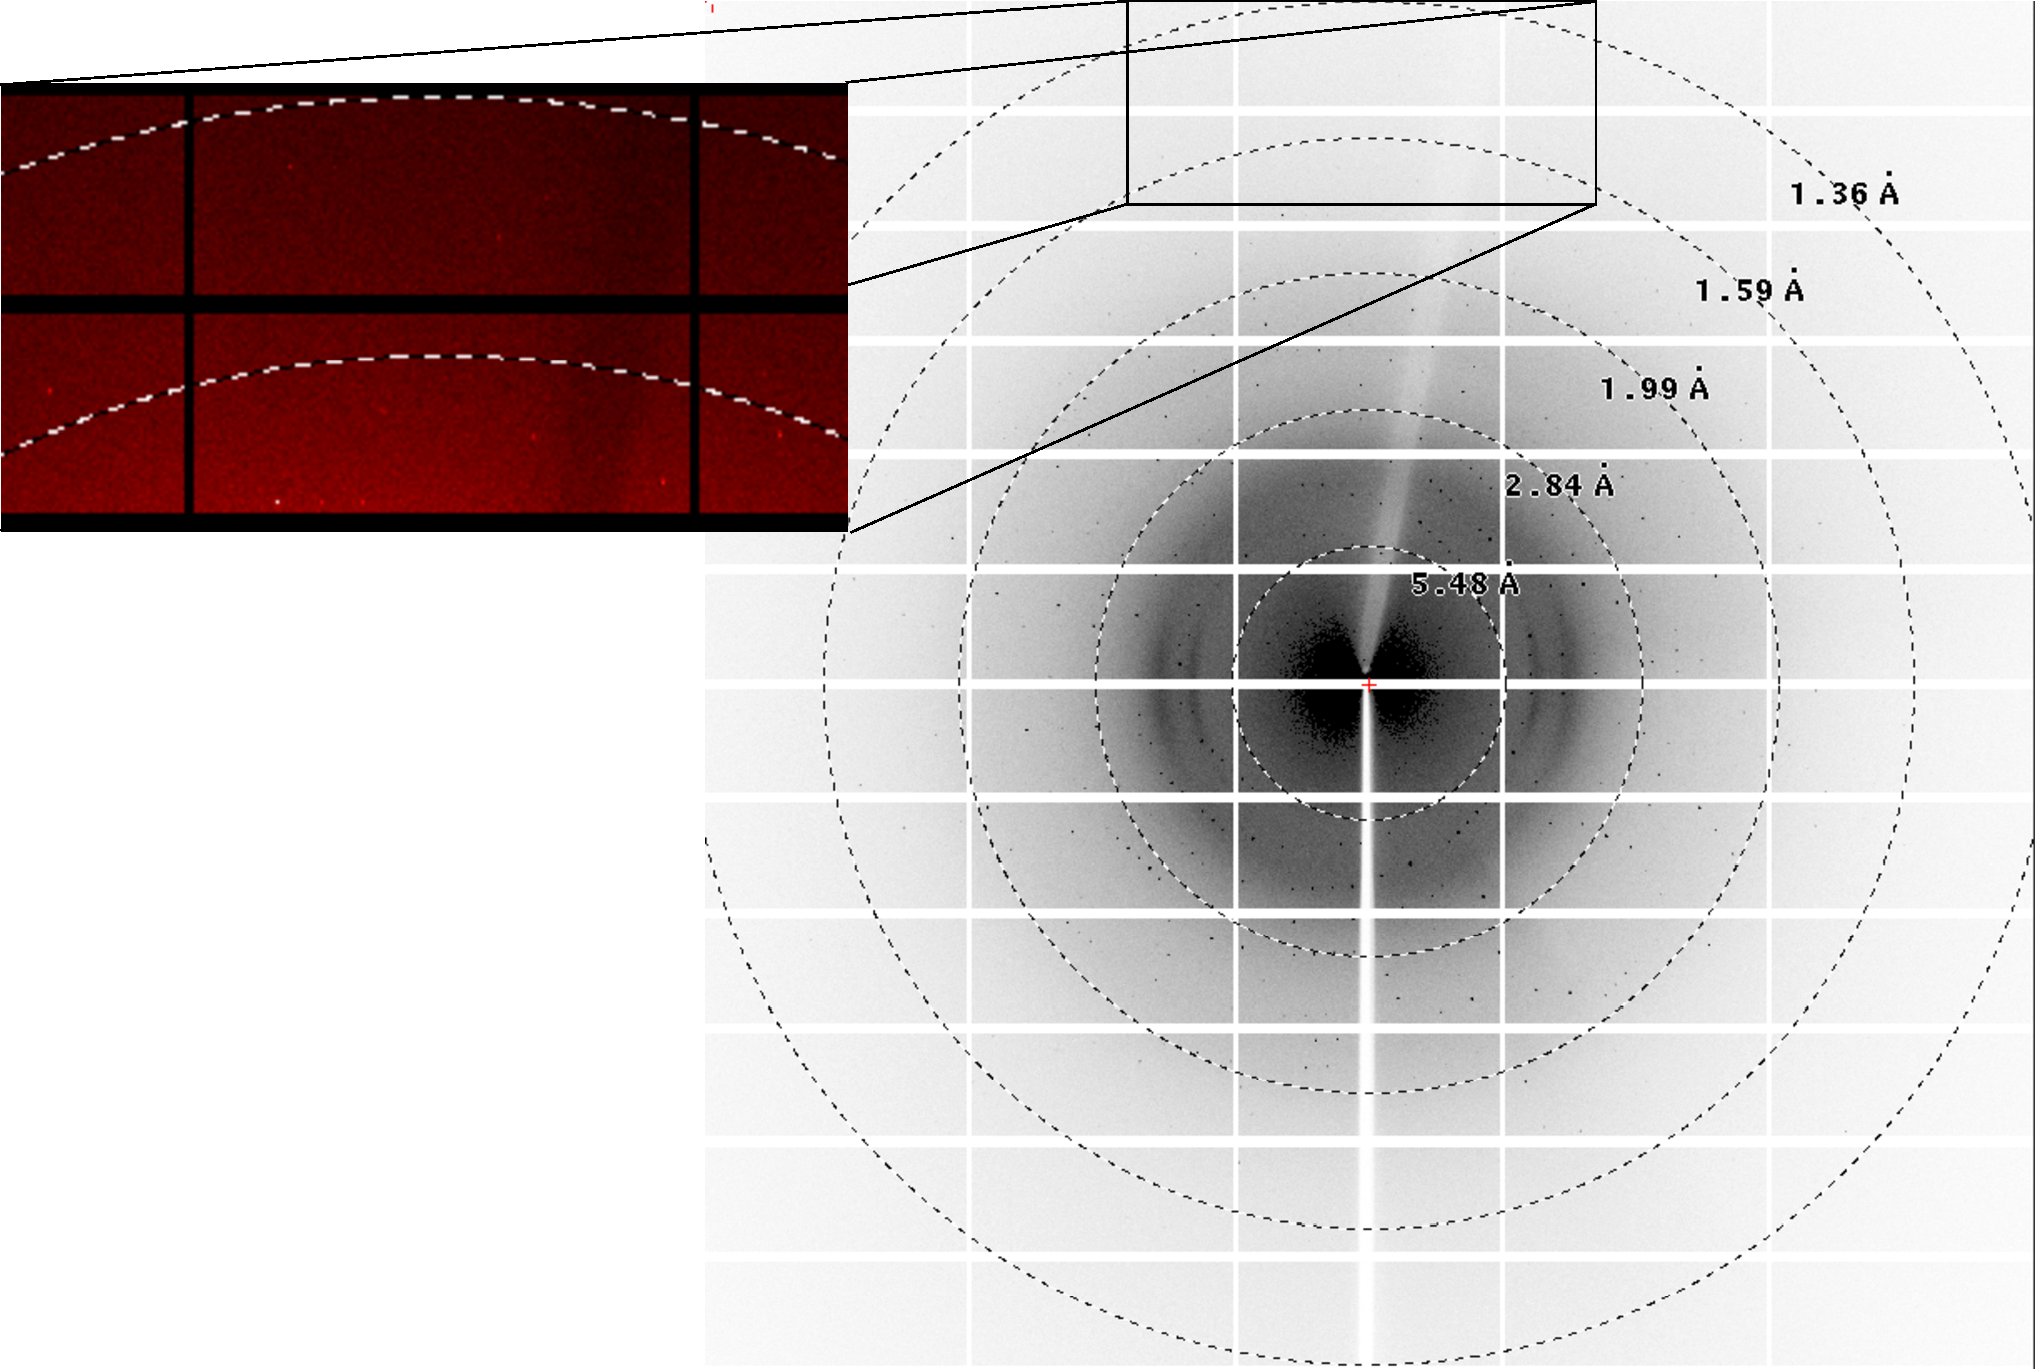
\includegraphics[width=1\textwidth]{figures/introduction/InsulinDiffractionImage.pdf}
            \caption[Insulin diffraction image.]{Diffraction image from a crystal of bovine pancreatic insulin crystallised in space group $I2_1 3$ recorded in January 2014 on beamline P14 at the PETRA III synchrotron, Hamburg.
            Inset: zoomed in section of the diffraction image with a `heat' colour scheme to improve visibility of the high resolution reflections.
            Individual spots known as reflections or Bragg peaks are clearly visible.}
            \label{fig:Insulin diffraction image}
        \end{figure}

    \subsection{Understanding diffraction from a crystal}
    \label{sub:Understanding diffraction from a crystal}

        \subsubsection{Scattering from a single electron}
        \label{subs:Scattering from single electron}
            The diffraction of the X-ray beam by the crystal results from the interaction of the electric component of the X-ray beam with the electrons in the crystal.
            When an X-ray hits an electron, the electron begins to oscillate.
            When the scattering is elastic (the desired scattering type for diffraction in MX), the original photon is absorbed by the electron which then emits an X-ray with the same wavelength as the incident X-ray photon, but with a phase shift of $180^{\circ}$.
            The amplitude of the electric component, $E_{el}$ of the scattered X-ray photon at a distance $r$ from a free (unbound) electron is given by
            \begin{equation}
                E_{el} = E_0 \f{1}{r}\f{e^2}{mc^2} \sin(\varphi),
            \end{equation}
            where $E_0$ is the amplitude of the electric vector of the incident X-ray photon, $e$ is the electron charge, $m$ is the electron mass, $c$ is the speed of light and $\varphi$ is the component of $E_0$ perpendicular to the scattering electron \cite{drenth2012}.

        \subsubsection{Scattering from a two electron system}
        \label{subs:Scattering from two electron system}
            Suppose a beam of X-rays is incident on a system of two electrons as depicted in Figure~\ref{fig:Two electron system}.
            \begin{figure}
                \centering
                \begin{subfigure}[b]{0.45\textwidth}
                        \centering
                        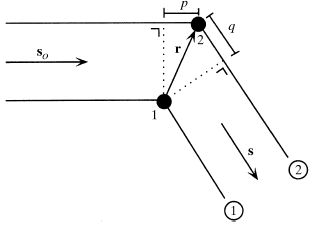
\includegraphics[width=\textwidth]{figures/introduction/twoelectronsystem.png}
                        \caption{}
                        \label{fig:Two electron system}
                \end{subfigure}
                \qquad
                \begin{subfigure}[b]{0.45\textwidth}
                        \centering
                        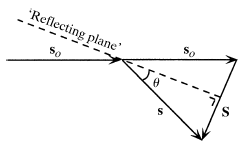
\includegraphics[width=\textwidth]{figures/introduction/scatteringvector.png}
                        \caption{}
                        \label{fig:scattering vector}
                \end{subfigure}
                \caption[X-ray scattering from two electrons.]{(a) Scattering from a system of two electrons labelled 1 and 2. Incident beam direction is denoted $\bs{s}_0$ and the scattered beam direction is denoted $\bs{s}$.
                The origin is defined at the position of electron 1. Electron 2 is at a position $\bs{r}$ with respect to electron 1.
                The path length difference of the beam scattered by electron 1 and electron 2 is $p + q$.
                (b) The angle $\theta$ is the angle between the incident beam and the reflecting plane.
                $\bs{S} = \bs{s} - \bs{s_0}$ and is perpendicular to the reflecting plane.
                The lengths of the vectors $\bs{s}$ and $\bs{s_0}$ are arbitrary but are chosen to be $1/\lambda$ for convenience, where $\lambda$ is the wavelength of the incident X-ray beam.
                This gives $|\bs{S}| = 2 \sin(\theta)/\lambda$ \cite{drenth1999}.}
        		\label{fig:Scattering from two electrons}
            \end{figure}
            The direction of the incident X-ray beam, $\bs{s}_0$, is altered after the diffraction event, and the direction of the scattered beam is denoted $\bs{s}$.
            The lengths of these vectors can be arbitrarily chosen.
            The convenient choice is $|\bs{s}| = |\bs{s}_0| = 1/\lambda$ where $\lambda$ is the wavelength of the incident beam.
            The path length difference of the beam scattered by electron 1 and electron 2 is $p + q = \lambda[\bs{r} \cdot (\bs{s}_0 - \bs{s})]$.
            Thus the second beam lags behind the first, and the resulting phase difference is
            \begin{equation}
                \f{-2 \pi}{\lambda} \times \lambda[\bs{r} \cdot (\bs{s}_0 - \bs{s})] = 2 \pi \bs{r} \cdot \bs{S},
            \end{equation}
            where $\bs{S} = \bs{s} - \bs{s_0}$ \cite{drenth1999}. Figure~\ref{fig:scattering vector} is a graphical description showing
            \begin{equation}
                |\bs{S}| = 2 \sin(\theta)/\lambda.
                \label{eq:length of vector S}
            \end{equation}
            where $\theta$ is the angle of reflection of the incident beam by the reflecting plane.
            It is important to note here that the phase of a wave with respect to a different wave is dependent on the relative position of the electrons.
            This demonstrates the importance of the phases for generating accurate structural information \cite{taylor2003phase, taylor2010}.

            The amplitudes of the scattered waves from both electrons in the system are the same, they only differ in phase.
            If the amplitude of the scattered wave from an electron positioned at the origing (e.g. electron 1) is equal to 1, then the total scattered wave from the two-electron system shown in Figure~\ref{fig:Two electron system} is $1 + 1 \times \exp[2 \pi i \bs{r} \cdot \bs{S}]$ where $i$ is the imaginary number, $i = \sqrt{-1}$.

        \subsubsection{Scattering from an atom}
        \label{subs:Scattering from an atom}
            The electron cloud of an atom scatters the incident X-ray beam.
            The strength of the scattered beam is dependent on the number of electrons and their positions in the electron cloud.
            The electrons in an atom are not free as was assumed in the original model of diffraction, but continuing to treat them as free electrons gives sufficient accuracy provided the wavelength of the incident beam is not too close to an absorption edge of the atom \cite{drenth2012}.
            Setting the origin of the system at the centre of the atom, the total scattering from the atom, $f$, is calculated as
            \begin{equation}
                f = \int_{\bs{r}} \rho(\bs{r}) \exp[2 \pi i \bs{r} \cdot \bs{S}]\ \mathrm{d}\bs{r},
                \label{eq:Atomic scattering factor all space}
            \end{equation}
            where $\rho(\bs{r})$ is the electron density at position $\bs{r}$ and the integral is over all space. $f$ is known as the atomic scattering factor \cite{drenth1999}.

            The electron density of an atom is assumed to be perfectly centrosymmetric i.e. $\rho(\bs{r}) = \rho(-\bs{r})$ (Figure~\ref{fig:atomic electron cloud}).
            Thus equation \ref{eq:Atomic scattering factor all space} can be simplified to
            \begin{equation}
                f = 2 \int_{\text{ half space}} \rho(\bs{r}) \cos[2 \pi \bs{r} \cdot \bs{S}]\ \mathrm{d}\bs{r}.
            \end{equation}
            The integral is only over half of the entire space and the quantity does not contain any imaginary terms, hence the atomic scattering factor is a real quantity.

            The atomic scattering factor of an atomic is only dependent on the length of the vector $\bs{S}$ (equation \ref{eq:length of vector S}).
            The dependence of the atomic scattering factor, $f$, on $|\bs{S}|$ is shown for carbon in Figure~\ref{fig:carbon atomic scattering factor}.

            \begin{figure}
                \centering
                \begin{subfigure}[b]{0.4\textwidth}
                        \centering
                        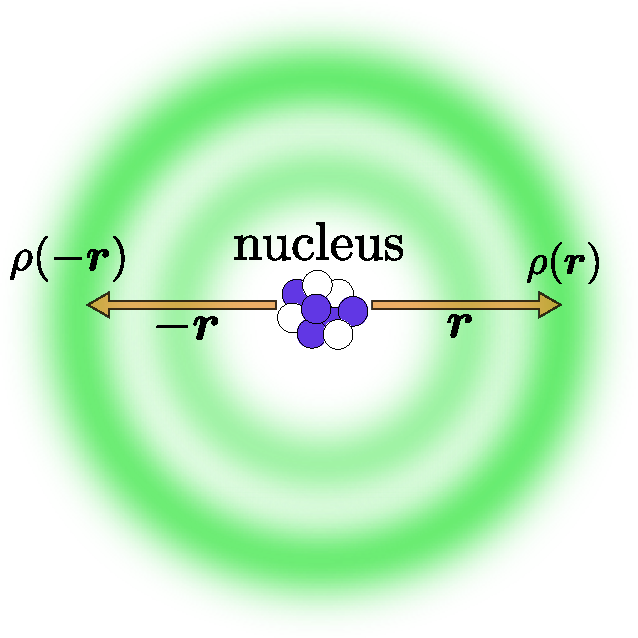
\includegraphics[width=\textwidth]{figures/introduction/atomicelectroncloud.pdf}
                        \caption{}
                        \label{fig:atomic electron cloud}
                \end{subfigure}
                \qquad
                \begin{subfigure}[b]{0.5\textwidth}
                        \centering
                        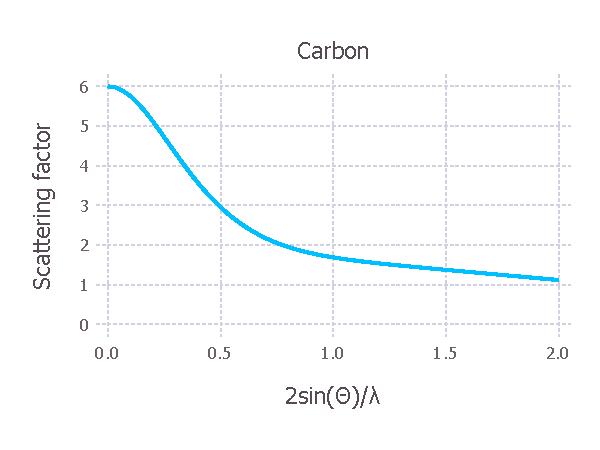
\includegraphics[width=\textwidth]{figures/introduction/carbonscatfac.pdf}
                        \caption{}
                        \label{fig:carbon atomic scattering factor}
                \end{subfigure}
                \caption[Centrosymmetric electron cloud and scattering factor from carbon]{(a) An atom with a centrosymmetric electron density distribution (i.e. $\rho(\bs{r}) = \rho(-\bs{r})$) about the centre of the nucleus.
                (b) atomic scattering factor, $f$, of carbon as a function of $|\bs{S}| = 2 \sin(\theta)/\lambda$.
                $f$ is expressed in number of electrons.
                Notice an angle of $\theta = 0$, $f=6$ corresponds to the atomic number of carbon.
                For this figure, $0^{\circ} \leq \theta \leq 90^{\circ}$ and $\lambda$ = 1.0$\,$\AA.}
        		\label{fig:Scattering from an atom}
            \end{figure}

        \subsubsection{Scattering from a unit cell}
        \label{subs:Scattering from a unit cell}
            Imagine an atom placed in a unit cell where the origin of the system is placed at the origin of the unit cell.
            Now the atom has positional vector $\bs{r}$ to define its location.
            The scattering from this atom is now
            \begin{equation}
                \bs{f} = f \exp[2 \pi i \bs{r} \cdot \bs{S}].
            \end{equation}
            Now suppose there are $N$ atoms in the unit cell. The total scattering from the unit cell is now
            \begin{equation}
                \bs{F}(\bs{S}) = \sum_{j=1}^N f_j \exp[2 \pi i \bs{r}_j \cdot \bs{S}].
                \label{eq:structure factor equation - summation}
            \end{equation}
            where $\bs{r}_j$ and $f_j$ are the position and atomic scattering factor of the $j$-th atom respectively.
            $\bs{F}(\bs{S})$ is referred to as the structure factor because it depends on the structure of the atoms within the unit cell \cite{drenth2012}.

        \subsubsection{Scattering from a crystal}
        \label{subs:Scattering from a crystal}
            Suppose an origin is chosen to be at the corner of an arbitrary unit cell but the scattering from a different unit cell from the same crystal is to be calculated.
            Unit cells are related by translations along the unit cell basis vectors $\bs{a}, \bs{b}$ and  $\bs{c}$ as described in section \ref{sub:Crystals}.
            So the unit cell of interest is located at position $t\bs{a} + u\bs{b} + v\bs{c}$, where $t,u,v \in \mathbb{Z}$ i.e. $t,u,v$ are integers.
            Thus the scattering from this unit cell is
            \begin{equation}
                \bs{F}(\bs{S}) \times \exp[2\pi i t\bs{a} \cdot \bs{S}] \times \exp[2\pi i u\bs{b} \cdot \bs{S}] \times \exp[2\pi i v\bs{c} \cdot \bs{S}].
            \end{equation}
            If this is extended to include all unit cells then the total wave scattered by the crystal is
            \begin{equation}
                \bs{K}(\bs{S}) \times \sum_{t=0}^{n_1}\exp[2\pi i t\bs{a} \cdot \bs{S}] \times \sum_{u=0}^{n_2}\exp[2\pi i u\bs{b} \cdot \bs{S}] \times \sum_{v=0}^{n_3}\exp[2\pi i v\bs{c} \cdot \bs{S}],
            \end{equation}
            where $n_1, n_2, n_3$ are the number of unit cells along the direction of the basis vectors $\bs{a}, \bs{b}$ and $\bs{c}$ respectively.
            Since $n_1, n_2$ and $n_3$ are typically very large, the summations
            $\sum_{t=0}^{n_1}\exp[2\pi i t\bs{a} \cdot \bs{S}]$, $\sum_{u=0}^{n_2}\exp[2\pi i u\bs{b} \cdot \bs{S}]$ and $\sum_{v=0}^{n_3}\exp[2\pi i v\bs{c} \cdot \bs{S}]$
            are usually equal to zero unless $\bs{a} \cdot \bs{S} = h$, $\bs{b} \cdot \bs{S} = k$ and $\bs{c} \cdot \bs{S} = l$ where $h,k,l \in \mathbb{Z}$.
            Therefore a crystal scatters X-rays if
            \begin{align}
                \bs{a} \cdot \bs{S} &= h, \\
                \bs{b} \cdot \bs{S} &= k, \\
                \bs{c} \cdot \bs{S} &= l.
                \label{eq:Laue conditions}
            \end{align}
            These are known as the Laue conditions \cite{drenth1999}. The $h,k,l \in \mathbb{Z}$ are referred to as Miller indices and they define individual reflections (Figure~\ref{fig:Insulin diffraction image}). The result is that the amplitude of the total scattered wave from the crystal is proportional to the structure factor $\bs{F}(\bs{S})$ and the number of unit cells in the crystal \cite{drenth1999}.

    \subsection{From diffraction patterns to electron density - The theory}
    \label{sub:From diffraction patterns to electron density - The theory}
        The goal of structure determination is to obtain the atomic structure of the target molecule.
        Therefore given that it is understood how X-ray diffraction arises from the interaction of X-rays with a crystal, the inverse problem must be solved i.e. determining the atomic structure from the diffraction pattern.

        Recalling equation \ref{eq:structure factor equation - summation} which allows the calculation of the structure factor as a summation over all atoms in the unit cell, it is possible to write this as an integral over the electron density in the cell instead, giving
        \begin{equation}
            \bs{F}(\bs{S}) = \int_{cell} \rho(\bs{r})\exp[2 \pi i \bs{r} \cdot \bs{S}]\ \mathrm{d}v.
            \label{eq:structure factor equation - integral}
        \end{equation}
        Introducing fractional coordinates $x, y, z$ (i.e. $0 \leq x < 1$ and similarly for $y$ and $z$) and given the unit cell has volume $V$, the volume element, $\mathrm{d}v$, can be rewritten as
        \begin{equation}
            \mathrm{d}v = V \times \mathrm{d}x\ \mathrm{d}y\ \mathrm{d}z.
        \end{equation}
        The position $\bs{r}$ can also be rewritten as $\bs{r} = \bs{a}x + \bs{b}y + \bs{c}z$, so this implies that
        \begin{align}
            \bs{r} \cdot \bs{S} &= \bs{a}\cdot\bs{S}\ x + \bs{b}\cdot\bs{S}\ y + \bs{c}\cdot\bs{S}\ z \\
            &= hx + ky + lz.
        \end{align}
        Thus $\bs{F}(\bs{S})$ can be written as a function of the Miller indices $\bs{F}(h,k,l)$ giving
        \begin{equation}
            \bs{F}(h,k,l) = V \int_{x=0}^1 \int_{y=0}^1 \int_{z=0}^1 \rho(x,y,z) \exp[2\pi i (hx + ky + lz)]\ \mathrm{d}x\ \mathrm{d}y\ \mathrm{d}z.
            \label{eq:structure factor equation - fractional integral}
        \end{equation}
        Equation \ref{eq:structure factor equation - fractional integral} shows explicitly that the structure factor $\bs{F}(h,k,l)$ is the Fourier transform of the electron density $\rho(x,y,z)$.
        Since the Fourier transform is the inverse of itself, it means that the electron density in the unit cell can be obtained by taking the Fourier transform of the structure factor
        \begin{equation}
            \rho(x,y,z) = \f{1}{V} \sum_h \sum_k \sum_l |\bs{F}(h,k,l)| \exp{-2\pi i (hx + ky + lz) + i \alpha(h,k,l)},
            \label{eq:electron density equation}
        \end{equation}
        where $|\bs{F}(h,k,l)|$ is the structure factor amplitude and $\alpha(h,k,l)$ is the phase. Equation \ref{eq:electron density equation} is known as the electron density equation and accurately calculating this is the ultimate goal of structure determination in MX.
        This is because it gives the density of electrons at every point in space in the unit cell.
        However, this equation can only be calculated once the amplitudes, $|\bs{F}(h,k,l)|$, and phases, $\alpha(h,k,l)$, are known.
        Notice that the summation is over reflections $(hkl$s$)$ which explains why it is desirable to accurately obtain as many reflections as possible in the data collection experiment.
        The more (accurate) $hkl$ terms that are used in the electron density equation, the better the Fourier series representation of the electron density in the unit cell (i.e. the better the electron density map).
        The amplitudes can be derived from the experimentally observed intensities in the data collection experiment but the phases are lost. This is known as the phase problem \cite{taylor2010}.

    \subsection{From diffraction patterns to electron density - In practice}
    \label{sub:From diffraction patterns to electron density - In practice}
        In practice, much of the theory is abstracted from the crystallographer and many software programs perform the necessary calculations `behind the scenes'.

        A set of diffraction images from a data collection experiment is known as a dataset. Extracting the amplitudes from the dataset is the ultimate aim of the first series of programs.
        The first step is to calculate the intensities of the observations from the images programs.
        Programs such as MOSFLM \cite{leslie2007}, XDS \cite{kabsch2010} and more recently DIALS \cite{waterman2013dials,waterman2016diffraction}, are used to find the spots on the images, determine the unit cell dimensions and its orientation with respect to the beam, assign Miller indices to each reflection (indexing) and finally integrate the intensity of the observations on the images.
        Commonly it is the case that a single observation is observed on multiple images because the rotation range of the crystal that results in a diffraction image (the oscillation angle) does not sample the entirety of a reflection.
        The fraction of the reflection that is recorded on a given image, the partiality of a reflection, has to be calculated and the experimental parameters refined in a process called post-refinement \cite{rossmann1979processing, rossmann1979oscillation}.

        Although the space group of the crystal is determined during the indexing stage, it is still only an informed prediction.
        An improvement of the predicted space group can be made after the integration stage with a ccp4 program called POINTLESS \cite{evans2011introduction}.

        The intensities of reflections are affected not only by the number of electrons in the unit cell, but also by the variation of other systematic factors such as the rotation rate, incident beam intensity, the path length of the X-ray beam through the crystal, and the secondary absorption etc. \cite{evans2005}.
        These factors must be taken into account so that the intensities of all reflections are on the same scale.
        To achieve this, the difference between intensities of reflections that should be identical according to the symmetry of the crystal are used to estimate the necessary parameters in a process called scaling.
        This is carried out by programs such as AIMLESS \cite{evans2013} and XSCALE \cite{kabsch2010}.

        Once the intensity estimates have been put on an internally consistent scale, it is possible to derive the amplitudes.
        In theory the amplitudes are equal to the square root of the intensities.
        However the conversion is not as straight forward as this, because subtraction of background noise in the diffraction images during the integration step leads to weakly measured intensity observations having negative values.
        This is a problem because it has been established that the amplitude should be a real quantity.
        One way to deal with negative intensity reflections is to set the intensity values to zero.
        However French and Wilson developed a treatment that uses Bayesian analysis \cite{french1978treatment} and Wilson statistics \cite{wilson1949probability} to calculate a better estimate of the amplitude given that a negative intensity has been observed.
        Programs such as CTRUNCATE \cite{evans2011introduction} perform this analysis and calculate further data assessment statistics to check for crystal pathologies such as twinning.

        Although phases are not observed directly in the diffraction experiment, they can be derived in multiple ways.
        If the sequence of the target protein is similar to another structure that has already been solved ($\approx$ 25-35\% \cite{taylor2010,abergel2013molecular}) or the structure is thought to be similar to another structure, then initial phases can be taken from the homologous structure.
        First, the homologue structure is transformed via a series of rotations and translations within the asymmetric unit of the target crystal so that the calculated amplitudes best match the ones that have been obtained experimentally \cite{mccoy2007solving}.
        Programs such as PHASER perform these operations \cite{mccoy2007phaser}.
        \newline
        If no structural homologue exists, then the phases must be derived experimentally.
        Isomorphous replacement is a method in which experimental data are collected on the native crystal and then again with a crystal in which a heavier element has been incorporated without changing the arrangement of the other atoms in the unit cells \cite{perutz1956isomorphous}.
        The phases can then be derived by analysing the difference in the intensity observations \cite{taylor2010}.
        \newline
        Another method known as anomalous dispersion can also be used, in which a heavy element is incorporated into the structure (sometimes this is not necessary if the structure already contains enough elements such as sulphur or heavier) and multiple datasets are collected at different X-ray photon energies.
        If possible, some of the datasets are collected at close to the absorption edge of the heavy element so appreciable differences between the native dataset and the new dataset can be measured \cite{bijvoet1954structure}.
        If only 1 dataset is collected, this is known as single wavelength anomalous dispersion (SAD) and differences in intensities are analysed between Friedel pairs ([h, k, l] and [-h, -k. -l]) of reflections.
        If datasets are collected at different incident X-ray energies, the method is known as multiple wavelength anomalous diffraction/dispersion (MAD) \cite{hendrickson1991determination,taylor2010}.
        \newline
        With both amplitudes and phases obtained, it is possible to perform the Fourier transform defined in equation \ref{eq:electron density equation} to obtain an electron density map.
        The atomic structure can then be built into the resulting map.
        In general the initial map is unlikely to provide a satisfactory structure, so a process of refinement is carried out to improve the agreement of the amplitude calculated from the model that has been built, with those that were derived from the experimental intensities.
        Programs such as REFMAC \cite{murshudov2011refmac5} and PHENIX.REFINE \cite{adams2010phenix} perform these operations until a satisfactory structure has been obtained.
        An atomic model is determined to be satisfactory when the statistical quantities, $R_{work}$ and $R_{free}$, are low enough.
        To ensure that the final structure is reliable, software programs such as MOLPROBITY \cite{chen2010molprobity} and PROCHECK \cite{laskowski1993procheck} are used to check the stereochemical quality of the structure.
